%%%%%latex preamble%%%%%
\documentclass[titlepage]{article}\usepackage[]{graphicx}\usepackage[]{color}
%% maxwidth is the original width if it is less than linewidth
%% otherwise use linewidth (to make sure the graphics do not exceed the margin)
\makeatletter
\def\maxwidth{ %
  \ifdim\Gin@nat@width>\linewidth
  \linewidth
  \else
  \Gin@nat@width
  \fi
}
\makeatother


\usepackage{listings}
\definecolor{mygreen}{rgb}{0,0.6,0}
\definecolor{mygray}{rgb}{0.5,0.5,0.5}
\definecolor{mymauve}{rgb}{0.58,0,0.82}
\lstset{ %
  backgroundcolor=\color{white},   % choose the background color; you must add \usepackage{color} or \usepackage{xcolor}
  basicstyle=\footnotesize,        % the size of the fonts that are used for the code
  breakatwhitespace=false,         % sets if automatic breaks should only happen at whitespace
  breaklines=true,                 % sets automatic line breaking
  captionpos=b,                    % sets the caption-position to bottom
  commentstyle=\color{mygreen},    % comment style
  deletekeywords={...},            % if you want to delete keywords from the given language
  escapeinside={\%*}{*)},          % if you want to add LaTeX within your code
  extendedchars=true,              % lets you use non-ASCII characters; for 8-bits encodings only, does not work with UTF-8
  frame=single,                    % adds a frame around the code
  keepspaces=true,                 % keeps spaces in text, useful for keeping indentation of code (possibly needs columns=flexible)
  keywordstyle=\color{blue},       % keyword style
  language=Python,                 % the language of the code
  morekeywords={*,...},            % if you want to add more keywords to the set
  numbers=left,                    % where to put the line-numbers; possible values are (none, left, right)
  numbersep=5pt,                   % how far the line-numbers are from the code
  numberstyle=\tiny\color{mygray}, % the style that is used for the line-numbers
  rulecolor=\color{black},         % if not set, the frame-color may be changed on line-breaks within not-black text (e.g. comments (green here))
  showspaces=false,                % show spaces everywhere adding particular underscores; it overrides 'showstringspaces'
  showstringspaces=false,          % underline spaces within strings only
  showtabs=false,                  % show tabs within strings adding particular underscores
  stepnumber=2,                    % the step between two line-numbers. If it's 1, each line will be numbered
  stringstyle=\color{mymauve},     % string literal style
  tabsize=2,                       % sets default tabsize to 2 spaces
  title=\lstname                   % show the filename of files included with \lstinputlisting; also try caption instead of title
}
\usepackage{alltt}
\usepackage[sc]{mathpazo}
\usepackage{amsmath, amsthm, amssymb}
\usepackage{graphicx}
\usepackage[T1]{fontenc}
\usepackage{geometry}
\geometry{verbose,tmargin=2.5cm,bmargin=2.5cm,lmargin=1.5cm,rmargin=1.5cm}
\setcounter{secnumdepth}{2}
\setcounter{tocdepth}{2}
\usepackage{url}
\usepackage[unicode=true,pdfusetitle,
  bookmarks=true,bookmarksnumbered=true,bookmarksopen=true,bookmarksopenlevel=2,
breaklinks=false,pdfborder={0 0 1},backref=false,colorlinks=false]
{hyperref}
\hypersetup{pdfstartview={XYZ null null 1}}
\usepackage{float}
\usepackage{bm}
\usepackage{tikz}
\usetikzlibrary{automata,arrows}
 %changes default sectioning commands -> 1,a, etc.
%\usepackage{breakurl}
\renewcommand{\thesubsection}{(\alph{subsection})}
\renewcommand{\thesubsubsection}{\roman{subsection}.}
\usepackage{lastpage}
\usepackage{fancyhdr}
\pagestyle{fancy}

%%% Header and Footer %%% 
\lhead{}
\chead{\leftmark}
\rhead{}
\lfoot{Aaron Gonzales; Theory of Computation}
\cfoot{Homework 1}
\rfoot{Page \thepage\ of \pageref{LastPage}}
\IfFileExists{upquote.sty}{\usepackage{upquote}}{}

\begin{document}

\title{Homework 1, CS500, Spring 2015}
\author{Aaron Gonzales}
\maketitle


%%%% useful align for this
\section{Exercise 1}
\begin{quote}
  \textbf{Show that the set of all langauges is uncountably infinite, while the
   set of DFAs is only countably infinite}
\end{quote}
\subsubsection{Answer:}
If we have an alphabet $\Sigma$ that is finite and non-empty, then $\Sigma^*$
is countably infinite as there is a bijection from $\Sigma^* \to \mathbb{N}$.
Cantor's theorem shows us that $\mathbb{N}$ has uncountably infinite subsets.

\section{Exercise 2}
\begin{quote}
  \textbf{Show that the the following languages are DFA-regular.
    \begin{itemize}
        \item The set of strings in ${a,b}∗$ with an even number of b's.
        \item The set of strings in ${a,b, c }∗$ where there is no c anywhere to the left of an a .
        \item The set of strings in ${0, 1}∗$ that encode, in binary, an
          integer w that is a multiple of 3. Interpret the empty string
          $\epsilon$ as the number zero.
      \end{itemize} 
  In each case, try to find the minimal DFA M, i.e., the one with the smallest
  number of states, such that $L = L(M)$.
  Offer some intuition about why you believe your DFA is minimal.}
\end{quote}
\subsubsection{Answer, 2.1}

  %%%%%% 2.2 answer %%%%%%%%%%%%
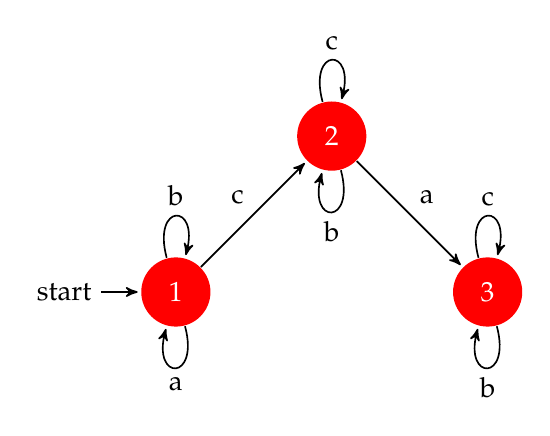
\begin{tikzpicture}[->,>=stealth',shorten >=1pt,auto,node distance=2.8cm,
                    semithick]
  \tikzstyle{every state}=[fill=red,draw=none,text=white]

  \node[initial,state] (A)                    {$1$};
  \node[state]         (B) [above right of=A] {$2$};
  \node[state]         (C) [below right of=B] {$3$};

  \path (A) edge              node {c} (B)
            edge [loop above] node {b} (A)
            edge [loop below] node {a} (A)
        (B) edge [loop above] node {c} (B)
        (B) edge [loop below] node {b} (B)
            edge              node {a} (C)
        (C) edge [loop above] node {c} (C)
            edge [loop below] node {b} (C);
\end{tikzpicture}

\subsubsection{Answer, 2.2}

  %%%%%% 2.2 answer %%%%%%%%%%%%
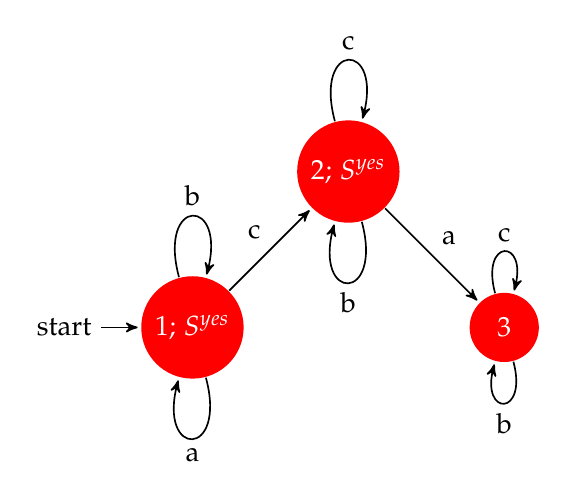
\begin{tikzpicture}[->,>=stealth',shorten >=1pt,auto,node distance=2.8cm,
                    semithick]
  \tikzstyle{every state}=[fill=red,draw=none,text=white]

  \node[initial,state] (A)                    {$1$; $S^{yes}$};
  \node[state]         (B) [above right of=A] {$2$; $S^{yes}$};
  \node[state]         (C) [below right of=B] {$3$};

  \path (A) edge              node {c} (B)
            edge [loop above] node {b} (A)
            edge [loop below] node {a} (A)
        (B) edge [loop above] node {c} (B)
        (B) edge [loop below] node {b} (B)
            edge              node {a} (C)
        (C) edge [loop above] node {c} (C)
            edge [loop below] node {b} (C);
\end{tikzpicture}


\subsubsection{Answer, 2.3}
  %%%%%% 2.3 answer %%%%%%%%%%%%
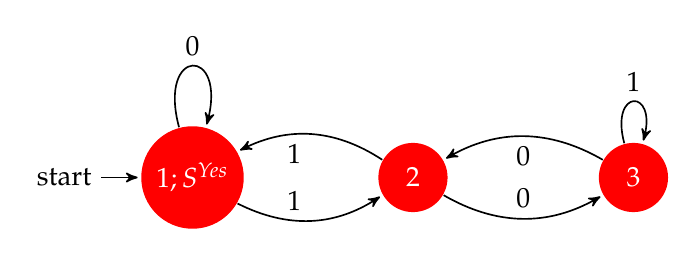
\begin{tikzpicture}[->,>=stealth',shorten >=1pt,auto,node distance=2.8cm,
                    semithick]
  \tikzstyle{every state}=[fill=red,draw=none,text=white]

  \node[initial,state] (A)                    {$1; S^{Yes}$};
  \node[state]         (B) [right of=A] {$2$};
  \node[state]         (C) [right of=B] {$3$};

  \path (A) edge [bend right] node {1} (B)
            edge [loop above] node {0} (A)
        (B) edge [bend right] node {1} (A)
            edge [bend right] node {0} (C)
        (C) edge [bend right] node {0} (B)
            edge [loop above] node {1} (C);
\end{tikzpicture}




\section{Show that any finite language is DFA Regular}
\begin{quote}
  \textbf{ }
\end{quote}
\subsubsection{Answer:}
We can show this via induction over the number of strings in the language.

Base case: $\epsilon$ is the empty string
Inductive Hypothesis: A finite language $L$ is comprised of finite strings

We know that if the string ${a}$ is regular then the string $L \cup {a}$ is
also regular and finite, by the IH. 

\section{Closure under complement}
\begin{quote}
  \textbf{Prove that if $L$ is DFA-regular, then $\bar{L}$ is DFA-regular.}
\end{quote}
\subsubsection{Answer:}

A DFA will make exactly one type of transition given input from a specific
state. Given DFA $M$ and language $L$, $w_1 \in L$, swapping accept and start
states of $M$, $L$ is not guarenteed to be recognized by $M$ any longer, though
as a DFA, $\bar{M}$ still can accept a regular language. Hence, regular
languages are closed (produce another set of the same set) under complement. 


\section{Closure under Union without DeMorgan}
\begin{quote}
  \textbf{If $L_1$ and $L_2$ are DFA regular, then $L_1 \cap L_2$ is DFA
  regular}
\end{quote}
\subsubsection{Answer:}
If we define a product automata $P$ of two automata $S,T$ with states $s_1,
s_2, \dots s_n$ and $t_1, t_2, \dots t_m$  as a resultant $P = ST$
to be the automata produced by the product of their individual states, such
that $P$ has state pairs $(s, t) $ with $ s \in S \text{and } t \in T$. A
product automata can be visualized as a matrix with row $S$ and column $T$.
This $P$ now recognizes the new language created by $S \cap T$. 

\section{Exercise 6}
\begin{quote}
  \textbf{Consider two DFAs, $M_1$ and $M_2$ with $n_1$ and $n_2$ states
  respectively. Show that if $L(M_1) \neq L(M_2)$ there is at least one word of
length less than $n_1n_2$ that $M_1$ accepts and $M_2$ rejects or vice versa.
Contrapositively, if all words of length less than $n_1n_2$ are given the same
response by both DFAs, they recognize the same language.}
\end{quote}
\subsubsection{Answer:}
  By making a product of $M_1$ and $M_2$\dots

\end{document}
